\documentclass[a4paper,headlines=4, footlines=1]{scrartcl}
\usepackage{amsmath,amssymb,amsthm,booktabs,braket,graphicx,hyphenat,lmodern,marginnote,microtype,scrpage2,tikz,tikz-3dplot}
\usepackage[utf8]{inputenc}
\let\marginpar\marginnote{}\usepackage[ngerman]{babel}\usepackage[german=quotes]{csquotes}\usepackage[T1]{fontenc}\usepackage{hyperref}\hypersetup{colorlinks=true,linkcolor=black,citecolor=black,filecolor=black,urlcolor=black}\newcommand{\E}{\mathrm{e}}\newcommand{\I}{\mathrm{i}}\newcommand{\de}{\mathrm{d}}\newcommand{\td}[2]{\frac{\de{#1}}{\de{#2}}}\pagestyle{scrheadings} \clearscrheadings\renewcommand{\headfont}{\normalfont}
%\lehead{\pagemark}
%\cehead{}
%\rehead{\headmark}
%\lohead{\rightmark}
%\cohead{}
%\rohead{\pagemark}
\setheadsepline{0.4pt}\setfootsepline{0.4pt}
\usepackage[inner=20mm,marginparsep=5mm,marginparwidth=30mm,outer=30mm,top=30mm,bottom=30mm,footskip=10mm]{geometry}
\usepackage[format=plain,margin=3em,font=small,labelfont=bf,labelsep=endash]{caption}
\renewcommand*{\marginfont}{\footnotesize} %\renewcommand{\vec}{\mathbf}
%\usepackage{kpfonts}
\usetikzlibrary{angles,quotes}

\usepackage{tabularx}
\usepackage{tkz-fct}

\addto\captionsngerman{%	
	\renewcommand{\figurename}{Abb.}	
	\renewcommand{\tablename}{Tab.}	
}

\ihead{Eberhard Karls Universität Tübingen\\
	Mathematisch-Naturwissenschaftliche Fakultät\\
	Fachdidaktik II: Geometrie\\
	Prof. Dr. Hermann Hähl}
\chead{}
\ohead{\parbox[l]{2.5cm}{A. Bucher\\
		P. Gepperth\\
		S. Jung\\
		J. Stigler}}

\ifoot{Sitzung 1: Strahlensätze}
\cfoot{}
\ofoot{\pagemark}


\title{Handout}

\subtitle{Strahlensätze}

\author{Pascal Gepperth}

\date{\today}

\hypersetup{
    pdftitle={Handout Fachdidaktik Mathematik Strahlensätze},
    pdfauthor={Pascal Gepperth},
	pdfstartview={FitH},
    pdfcreator={LaTeX with TikZ}
}



\begin{document}

\section{Fachwissenschaftliche Auffassung}
% Vorüberlegung
\begin{minipage}{.5\textwidth}
	Inhalt...
\end{minipage}
\begin{minipage}{.5\textwidth}
	\begin{tikzpicture}[thick]
		% lines
		\draw (7,0) -- (0,0) -- (5,5);
		\draw (3,-1) -- ({3-2*.6},{-1+7*.6});
		\draw (4,-1) -- ({4-2*.7},{-1+7*.7});
		\draw (5,-1) -- ({5-2*.8},{-1+7*.8});
		% triangles
		\draw ({3-2*.143},{-1+7*.143}) -- ({3-2*.143 + .78},{-1+7*.143 + .78});
		\draw ({4-2*.143},{-1+7*.143}) -- ({4-2*.143 + .78},{-1+7*.143 + .78});
		% angles
		\draw ({3-2*.143+.35},{-1+7*.143}) arc[radius = .7cm, start angle = 0, end angle = 25];
		\draw ({4-2*.143+.35},{-1+7*.143}) arc[radius = .7cm, start angle = 0, end angle = 25];
		\draw (.35,0) arc[radius = .7cm, start angle = 0, end angle = 25];
		
		\draw ({3-2*.143 + .78-.2},{-1+7*.143 + .78-.2}) arc[radius = .5cm, start angle = 220, end angle = 260];
		\draw ({4-2*.143 + .78-.2},{-1+7*.143 + .78-.2}) arc[radius = .5cm, start angle = 220, end angle = 260];
		% congs
		\draw[thin] (.3,.15) -- (.4,.15);
		\draw[thin] (3.0,.15) -- (3.1,.15);
		\draw[thin] (4.0,.15) -- (4.1,.15);
		
		\draw[thin] (3.2,3.1) -- (3.2,3.3);
		\draw[thin] (3.25,3.15) -- (3.25,3.35);
		\draw[thin] (2.4,2.3) -- (2.4,2.5);
		\draw[thin] (2.45,2.35) -- (2.45,2.55);
		\draw[thin] (3.2,0.4) -- (3.2,0.6);
		\draw[thin] (3.15,0.35) -- (3.15,0.55);
		\draw[thin] (4.2,0.4) -- (4.2,0.6);
		\draw[thin] (4.15,0.35) -- (4.15,0.55);
		% nodes
		\node at ({3-2*.6+.2},{-1+7*.6}) {g};
		\node at ({4-2*.7+.2},{-1+7*.7}) {h};
		\node at ({5-2*.8+.2},{-1+7*.8}) {i};
	\end{tikzpicture}
\end{minipage}

% Erster Strahlensatz, kommensurabel
\begin{minipage}{.5\textwidth}
	\begin{tikzpicture}
		\draw[thick] (7,0) -- (0,0) -- (5,5);
		\draw[thick] (3,-1) -- ({3-2*.7},{-1+7*.7});
		\draw (2,-1) -- ({2-2*.5},{-1+7*.5});
		\draw (1,-1) -- ({1-2*.4},{-1+7*.4});
		\draw (5,-1) -- ({5-2*.8},{-1+7*.8});
		\draw (4,-1) -- ({4-2*.7},{-1+7*.7});
		\draw[thick] (6,-1) -- ({6-2},{-1+7});

		\node at (2.1,3) {g};
		\node at (4.35,5.5) {h};
		\node at (.8,1.25) {$\varepsilon_1$};
		\node at (1.25,-.3) {$\varepsilon_2$};
		
		\draw [decorate,decoration={brace,amplitude=10pt},xshift=-4pt,yshift=0pt]
		({0-2*.5+.5},{-1+7*.5-1}) -- ({3-2*.7+.1},{-1+7*.7-1*.7/1.1}) node [black,midway,xshift=-0.3cm,yshift=.4cm] 
		{$m$};
		\draw [decorate,decoration={brace,amplitude=10pt},xshift=-4pt,yshift=0pt]
		({0-2*.5},{-1+7*.5}) -- ({6-2*1.1},{-1+7*1.1}) node [black,midway,xshift=-0.3cm,yshift=.4cm] 
		{$n$};
		
		\draw [decorate,decoration={brace,amplitude=10pt,mirror,raise=4pt},yshift=0pt]
		(0,-1) -- (3,-1) node [black,midway,yshift=-.7cm] {$m$};
		\draw [decorate,decoration={brace,amplitude=10pt,mirror,raise=4pt},yshift=0pt]
		(0,-1.6) -- (6,-1.6) node [black,midway,yshift=-.7cm] {$n$};
	\end{tikzpicture}
\end{minipage}
\begin{minipage}{.5\textwidth}
	Inhalt...
\end{minipage}
\section{Schulische Auffassung}
Beweise durch Gegenbeispiele bieten eine schöne Möglichkeit "`universitätsnahe`` Mathematik für SuS zugänglich zu machen. Im Falle der Umkehrungen der Strahlensätze ist dies eine anspruchsvolle (aber nicht unmögliche) Aufgabe an Lehrkraft und SuS. Darum lassen sich die Umkehrungen auch nicht in jedem Schulbuch finden. \\
Dennoch scheint die Thematik prädestiniert für das entdeckende Lernen zu sein. So z.B. im Falle der Umkehrung des 2. Strahlensatzes:\\
\begin{minipage}{0.5\textwidth}
	\textit{Finde mit Zirkel und Geodreieck eine Situation, in welcher $\frac{|SA_1|}{|SA_2|}=\frac{|A_1B_1|}{|A_2B_2|}$ gilt, aber g und h nicht parallel sind.}	
\end{minipage}
\begin{minipage}{0.5\textwidth}
	\begin{flushright}
		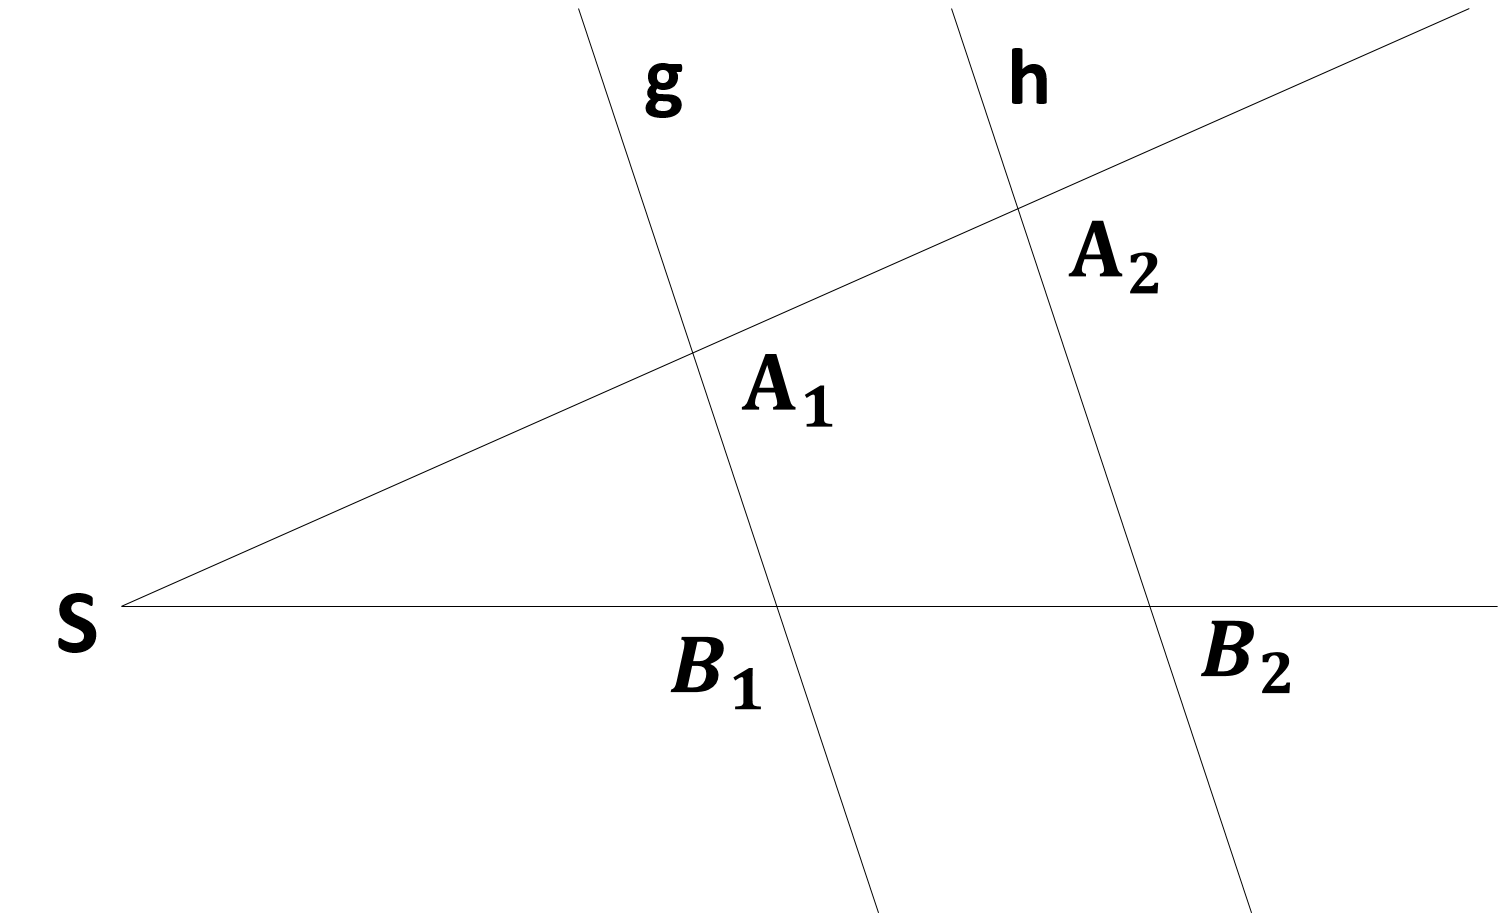
\includegraphics[scale=0.15]{Skizze}
	\end{flushright}
\end{minipage}\\
Folgende anspruchsvolle Aufgabe wurde in einem Schulbuch (Elemente der Mathematik) gestellt:\\
\textit{Nach dem ersten erweiterten Strahlensatzes gilt auch:}
\begin{align}
\text{Wenn } g\parallel h\text{, dann gilt } \frac{|SA_1|}{|A_1A_2|}=\frac{|SB_1|}{|B_1B_2|} 
\end{align}
\textit{Gib den Kehrsatz an und widerlege ihn.}

\end{document}
